\let\negmedspace\undefined
\let\negthickspace\undefined
\documentclass[journal,12pt,onecolumn]{IEEEtran}
\usepackage{cite}
\usepackage{amsmath,amssymb,amsfonts,amsthm}
\usepackage{algorithmic}
\usepackage{graphicx}
\graphicspath{{./figs/}}
\usepackage{textcomp}
\usepackage{xcolor}
\usepackage{txfonts}
\usepackage{listings}
\usepackage{enumitem}
\usepackage{mathtools}
\usepackage{gensymb}
\usepackage{comment}
\usepackage{caption}
\usepackage[breaklinks=true]{hyperref}
\usepackage{tkz-euclide} 
\usepackage{listings}
\usepackage{gvv}                                        
%\def\inputGnumericTable{}                                 
\usepackage[latin1]{inputenc}     
\usepackage{xparse}
\usepackage{color}                                            
\usepackage{array}                                            
\usepackage{longtable}                                       
\usepackage{calc}                                             
\usepackage{multirow}
\usepackage{multicol}
\usepackage{hhline}                                           
\usepackage{ifthen}                                           
\usepackage{lscape}
\usepackage{tabularx}
\usepackage{array}
\usepackage{float}

\begin{document}

\title{9.2.34}
\author{AI25BTECH11001 - ABHISEK MOHAPATRA}
{\let\newpage\relax\maketitle}
	
	 	\textbf{Question}:
Find the area of region bounded by the line $x = 2$ and the parabola $y^2 = 8x$.

		\textbf{Solution:}

	Graph:
\begin{figure}[h!]
	\centering
	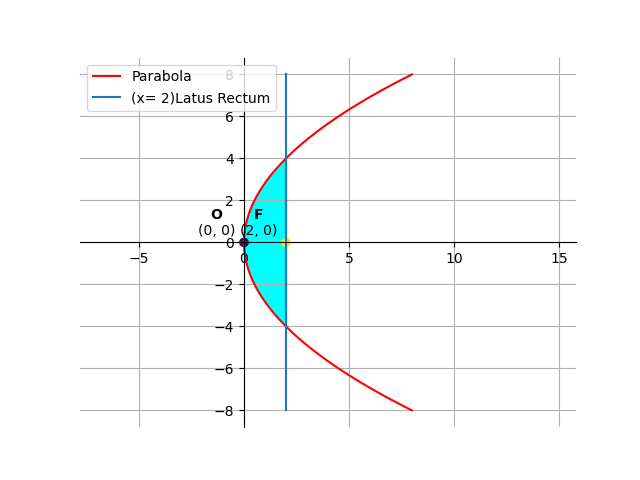
\includegraphics[width=0.7\linewidth]{img.png}
\end{figure}

From the given information, the parameters of the parabola and line are
\begin{align}
		\vec{V} = \myvec{0&0\\0&1}, \vec{u} = \myvec{-4\\0} , f = 0, \vec{h} =\myvec{2\\0}, \vec{m}=\myvec{0\\1} 
\end{align}
Substituting from the above in (9.1.1.3),
\begin{align}
k_i=4,-4
\end{align}
yilelding the points of intersection
\begin{align}
		\vec{a_0}=\myvec{2\\4},\vec{a_1}=\myvec{2\\-4}
\end{align}
Thus, the area of the parabola in between the lines $x = 2$ is given by
\begin{align}
\int_0^2 \sqrt{8x} = \frac{16}{3}
\end{align}


\end{document}



